\documentclass[aps,pre,twocolumn,superscriptaddress,floatfix,nofootinbib]{revtex4-2}

\usepackage{amsmath,amssymb}
\usepackage{graphicx}
\usepackage{bm}
\usepackage[colorlinks=true,allcolors=blue]{hyperref}

\begin{document}

\title{Triadic closure and opening decoupled from growth: condensation and a tree phase}

\author{Alexei V\'azquez}

\date{\today}

\begin{abstract}
In the local-search model $LS(n,1)$ a newcomer links to a random node and to
one of its neighbours, so every arrival closes a triangle. We decouple the two
acts: nodes arrive at rate $\alpha$ and attach to a random node, and open triads
close at rate $\beta_+$. Because $\alpha+\beta_+$ only sets the clock, the model has
one parameter, $u=\beta_+/(\alpha+\beta_+)$. Holding the two total rates in fixed
ratio is the only choice that keeps the mean degree constant,
$\langle k\rangle=2/(1-u)$, and $\alpha=\beta_+$ reproduces the density of
$LS(n,1)$. If instead each open triad closes at its own rate, the mean degree
diverges in finite size for every $\beta_+/\alpha$ we have simulated. The
interesting part is how the triad is chosen. If the closing triad is drawn
uniformly from all open triads --- a rule that needs a census of the whole
network --- the network condenses. Beyond an onset size $n^*(u)$ a near-clique
core of order $\sqrt n$ nodes, with degrees of order $\sqrt n$, captures a
finite fraction of all links. The onset size grows steeply as $u\to0$, roughly
as $u^{-5}$, and we find no threshold down to $u=0.08$. Local implementations of
the same closure (a random node introducing two of its friends, or befriending
a friend of a friend) stay in the normal, scale-free phase. The
friend-of-a-friend version at $u=1/2$ recovers the exponent $\gamma=5$ of
$LS(n,1)$. Adding the reverse process, the removal of a link of a closed triad
at rate $\beta_-$, gives a phase diagram with three phases. For
$\beta_-\ge\beta_+$ removals are limited by the triangles available, every
triangle is opened soon after it forms, and the network stays a tree with
$\langle k\rangle=2$ and bounded degrees. For $\beta_-<\beta_+$ the density is
$\langle k\rangle=2[1+(\beta_+-\beta_-)/\alpha]$. Moderate turnover dilutes the
condensate into a sparse club of $n^{a}$ nodes, $a<1$, that still holds every net
closure link. Turnover above $\beta_-/\beta_+\approx0.83$ dissolves it, leaving a
hub-free network with triangles.
\end{abstract}

\maketitle

%=====================================================================
\section{Introduction}

Triadic closure --- a link forming between two nodes that share a neighbour ---
is the mechanism behind the high clustering of social networks
\cite{granovetter1973,davidsen2002,holme2002,vazquez2003,toivonen2006,jackson2007}.
In the local-search model $LS(n,\ell)$ \cite{vazquez2001,vazquez2003,book} with
$\ell=1$, a newcomer picks a random node $j$, links to it, and links to a random
neighbour of $j$. Every arrival therefore closes exactly one triangle, and
arrival and closure are the same event.

In real social systems they are not. People join at one rate, and introductions
among people already present happen at another. The natural generalization runs
two processes side by side: \emph{node addition}, at total rate $\alpha$, in
which a new node attaches to a uniformly random node; and \emph{closure}, at
total rate $\beta_+$, in which a randomly selected open triad
--- a path $a$--$c$--$b$ with $a$ and $b$ unlinked --- is closed by the link
$(a,b)$.

Two questions arise. The first is how to choose $\alpha$ and $\beta_+$, given that
$\alpha+\beta_+$ only sets the time scale and that the mean degree must stay
constant (Sec.~\ref{sec:rates}). The second is what the decoupled rule builds.
The answer depends on what ``randomly selected'' means. Drawing the triad
uniformly from all open triads produces a condensation transition
(Sec.~\ref{sec:condensation}) absent from every local implementation of the same
closure (Sec.~\ref{sec:normal}). Finally, we add the reverse of closure: at rate
$\beta_-$ a closed triad is opened by removing one of its links
(Sec.~\ref{sec:opening}).

%=====================================================================
\section{The choice of $\alpha$ and $\beta_+$}
\label{sec:rates}

Measure time by events and let $u=\beta_+/(\alpha+\beta_+)$ be the probability that
an event is a closure; $r_+=\beta_+/\alpha=u/(1-u)$ is the number of closures per
arrival. Each arrival adds one node and one link, and each closure adds one
link. After $n$ arrivals, $E=n(1+r_+)$, so
\begin{equation}
  \langle k\rangle=\frac{2E}{n}=2(1+r_+)=\frac{2}{1-u}
  \qquad\Leftrightarrow\qquad
  \frac{\beta_+}{\alpha}=\frac{\langle k\rangle}{2}-1 .
  \label{eq:kmean}
\end{equation}
Every arrival in $LS(n,1)$ adds one node and two links, so $\langle k\rangle=4$.
The decoupled model has the same density at $\beta_+=\alpha$, $u=1/2$. Any fixed
ratio gives a constant $\langle k\rangle$, which is exact in the large-$n$ limit
whatever the closure rule.

The alternative reading makes the rates per capita: each node spawns newcomers
at rate $\alpha$ and each open triad closes at rate $\beta_+$. The closure rate is
then $\beta_+ W$, with $W$ the number of open triads, and $W/n$ is not a
constant of the dynamics. Section~\ref{sec:pertriad} shows that this version has
no stationary $\langle k\rangle$. Fixing the ratio of the total rates is
therefore the only consistent choice, and we use it throughout. With triad
opening at total rate $\beta_-$ (Sec.~\ref{sec:opening}) the condition becomes
$\beta_+-\beta_-=\alpha(\langle k\rangle/2-1)$, which can hold only for
$\beta_+>\beta_-$.

%=====================================================================
\section{Closure rules and their mean-field exponents}
\label{sec:normal}

We compare four ways to pick the pair to be closed, all at the same $u$:
\begin{itemize}
\item[(w)] \emph{random open triad}: uniform over all open triads $a$--$c$--$b$.
  The centre is chosen with probability $\propto k_c(k_c-1)$, so this rule
  needs a census of the network.
\item[(p)] \emph{random potential link}: uniform over unlinked pairs with at
  least one common neighbour. This is the rule simulated in
  Ref.~\cite{book}, Ch.~3. It differs from (w) only in that a pair with $m$
  common neighbours is not $m$ times likelier.
\item[(c)] \emph{introducer}: a uniformly random node $c$ with $k_c\ge 2$ links
  two random neighbours of its own. This is local.
\item[(f)] \emph{friend of a friend}: a uniformly random node $a$ walks two steps,
  $a\to j\to l$, and links to $l$. This is local.
\end{itemize}
If the selected pair is already linked, the draw is repeated.

\paragraph*{Mean field.}
Neglect degree correlations and let each closure pick $e$ of its two endpoints
with probability $\propto k$ and the other $2-e$ uniformly. A node then gains
links at rate
\begin{equation}
  n\frac{dk_i}{dn}=1+r_+(2-e)+\frac{r_+\,e}{\langle k\rangle}\,k_i
  =1+r_+(2-e)+\frac{e\,u}{2}\,k_i ,
  \label{eq:mf}
\end{equation}
where we used Eq.~\eqref{eq:kmean}. The density cancels out of the preference.
Hence $k_i\sim(n/n_i)^{b}$ with $b=e u/2$, and $\gamma=1+1/b$:
\begin{equation}
  \gamma=1+\frac{2}{e\,u}.
  \label{eq:gamma}
\end{equation}
Rules (w), (c) and (p) close a pair whose two endpoints are both reached through
a link, so $e=2$ and $\gamma=1+1/u$. At $u=1/2$ this gives $\gamma=3$. Rule (f)
starts from a uniformly random node, so $e=1$ and $\gamma=1+2/u$. At $u=1/2$
this gives $\gamma=5$, which equals the exponent of $LS(n,1)$ itself
\cite{book}. That model has $b=1/\langle k\rangle=1/4$: its newcomer is the
uniform endpoint and the neighbour of $j$ the preferential one. Decoupling
arrival from closure does not change the exponent so long as the closure keeps
one endpoint uniform.

\begin{figure}[t]
\includegraphics[width=\columnwidth]{fig-rules.pdf}
\caption{Five rules at the same density, $\langle k\rangle=4$ ($u=1/2$),
$n=10^6$. (a) Cumulative degree distribution. (b) Mean degree of nodes against
their age $\tau=n/n_i$. The two local rules and $LS(n,1)$ grow as power laws. The
two census rules saturate for the oldest nodes, which have condensed into a
core.}
\label{fig:rules}
\end{figure}

\paragraph*{Simulations.}
Figure~\ref{fig:rules} and Table~\ref{tab:rules} compare the rules at $u=1/2$,
$n=10^6$. The two local rules behave as Eq.~\eqref{eq:gamma} says, up to the
corrections expected from correlations and from a window of only five decades:
the age exponent $b$ is $0.31$ for (f) (mean field $1/4$) and $0.37$ for (c)
(mean field $1/2$), against $0.27$ for $LS(n,1)$ (exact $1/4$). They keep high
mean local clustering, $\bar C\approx0.4$, and are mildly assortative. The two
census rules are qualitatively different. The oldest nodes' degree saturates
(Fig.~\ref{fig:rules}b), the distribution develops a hump at large $k$
(Fig.~\ref{fig:rules}a), and a few hundred to a few thousand nodes carry a
large share of the links. That is the condensation of the next section.

\begin{table}[b]
\caption{Rules at $u=1/2$, $n=10^6$, one realization. $b$: age exponent
(fit over $10^2<n_i<10^5$); $b_{\rm MF}=eu/2$; $\mathcal T$: transitivity;
$\bar C$: mean local clustering; $r_k$: degree assortativity; $\phi$: fraction of
links with both ends among the $\sqrt n$ highest-degree nodes; $\rho$: density
of that core.}
\label{tab:rules}
\begin{ruledtabular}
\begin{tabular}{lccccccc}
rule & $b$ & $b_{\rm MF}$ & $k_{\max}$ & $\mathcal T$ & $\bar C$ & $r_k$ & $\phi\ (\rho)$\\
\hline
$LS(n,1)$ & 0.27 & 1/4 & 169 & 0.25 & 0.69 & 0.05 & 0.001 (0.002)\\
(f) & 0.31 & 1/4 & 203 & 0.24 & 0.37 & 0.28 & 0.002 (0.008)\\
(c) & 0.37 & 1/2 & 391 & 0.22 & 0.42 & 0.16 & 0.002 (0.007)\\
(p) & 0.66 & 1/2 & 684 & 0.03 & 0.02 & 0.52 & 0.026 (0.11)\\
(w) & 0.89 & 1/2 & 1619 & 0.48 & 0.008 & 0.65 & 0.20 (0.81)\\
\end{tabular}
\end{ruledtabular}
\end{table}

%=====================================================================
\section{Condensation under uniform triad selection}
\label{sec:condensation}

\paragraph*{The condensed phase.}
Under rule (w) at $u=1/2$ and $n=10^6$, the $10^3=\sqrt n$ highest-degree nodes
are linked to one another with density $0.81$ and hold $20\%$ of all links.
The 100 richest form a complete graph. All of them were born among the first
few thousand arrivals. The core's share of the links does not shrink with
size: $\phi=0.176$, $0.192$, $0.202$ at $n=10^4,10^5,10^6$, while its density
climbs to $0.71$, $0.77$, $0.81$. The same holds for every $u\ge0.3$
(data/scan.csv). The core is a dense block of $\Theta(\sqrt n)$ nodes inside a
sparse network. The number of triangles therefore grows as $T\sim n^{3/2}$, and
the global transitivity stays near $0.5$ while the mean local clustering
vanishes, because the bulk of degree-one newcomers is never closed.

The hub degree follows from the core's own wedges. Once core-centred triads
dominate $W$, a core node $a$ is an endpoint of a closure with probability
$\simeq w_a/W$. Here $w_a\simeq\rho\sqrt n\,K$ (a triad through any of its
$\rho\sqrt n$ core neighbours) and $W\simeq\sqrt n\,K^2/2$. Hence
$n\,dK/dn\simeq 2\rho r_+ n/K$, giving
\begin{equation}
  K^2\simeq c\,r_+\,n ,
  \label{eq:K}
\end{equation}
with $c$ of order $4\rho$. The data give $k_{\max}^2/(r_+n)=2.8$, $2.7$, $2.6$,
$2.5$ at $u=0.3$--$0.6$ ($n=10^6$), drifting down by about $10\%$ per decade
($2.4$ at $u=1/2$, $n=8\times10^6$).
In Fig.~\ref{fig:transition}b this is the plateau of $k_{\max}/\sqrt N$.

\begin{figure*}[t]
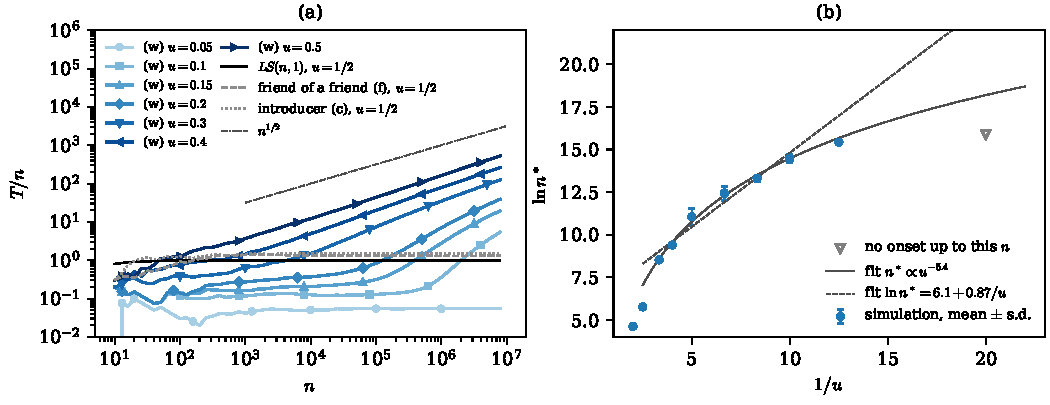
\includegraphics[width=\textwidth]{fig-transition.pdf}
\caption{The condensation transition under uniform triad selection (rule w).
(a) Triangles per node and (b) $k_{\max}/\sqrt N$ along single trajectories up
to $N=10^7$. In the normal phase $T/N$ is constant and $k_{\max}/\sqrt N$
falls. In the condensed phase $T/N\propto N^{1/2}$ and $k_{\max}/\sqrt N$ is
constant. The local rules (grey; $u=1/2$) stay normal. (c) Onset size $n^*$
(first $N$ with $T/N\ge1$), mean and spread over 5--6 seeds for
$0.1\le u\le0.25$, one trajectory otherwise. The lines are fits over
$0.1\le u\le0.3$. The triangle marks the largest size reached without onset
($u=0.05$, $N=10^7$). The point at $1/u=12.5$ is from two runs to
$3\times10^7$ and was not used in the fits.}
\label{fig:transition}
\end{figure*}

\paragraph*{Onset.}
Figure~\ref{fig:transition} follows single trajectories to $N=10^7$. For
$u\ge0.3$ the network condenses within a few hundred to a few thousand
arrivals. At smaller $u$ there is a long normal plateau --- $T/N$ constant and
$k_{\max}/\sqrt N$ falling --- that ends abruptly: $T/N$ turns up and
$k_{\max}/\sqrt N$ rises back to its condensed value. Taking the onset size
$n^*$ as the first $N$ with $T/N\ge1$, we find
\begin{center}
\begin{tabular}{lcccccc}
$u$ & 0.08 & 0.10 & 0.12 & 0.15 & 0.20 & 0.25\\
$\ln n^*$ & 15.4 & 14.5 & 13.3 & 12.4 & 11.1 & 9.4\\
\end{tabular}
\end{center}
with seed-to-seed spread $0.1$--$0.5$ (5--6 seeds per $u$ for
$0.1\le u\le0.25$). Over $0.1\le u\le0.3$ a power law, $n^*\propto u^{-5.4}$,
fits with rms $0.17$ in $\ln n^*$. An essential singularity,
$\ln n^*=6.1+0.87/u$, fits with rms $0.41$. Fitted before the $u=0.08$ runs
existed, these two forms predicted $\ln n^*=15.7$ and $17.0$ for $u=0.08$. Two
runs to $3\times10^7$ both condensed at $\ln n^*=15.4$; five runs stopped at
$3\times10^6$ had not yet condensed, as both forms require. The power law is
therefore preferred. Plotted against $1/u$, the onset curve bends down, not
up. A finite threshold $u_c>0$,
at which $n^*$ would diverge, would bend it up. At $u=0.05$ nothing happens up
to $10^7$; the power law puts the onset at $n^*\approx8\times10^7$.

The evidence thus favours a transition at $u_c=0$: in the limit $n\to\infty$,
any positive closure rate condenses the network under uniform triad selection.
The approach is so slow, however, that for $u\lesssim0.05$ the normal phase is
what any realistic size shows. We cannot exclude a threshold below $u=0.08$.

\paragraph*{Mechanism.}
Under rule (w) a node becomes the endpoint of a closure with probability
$w_a/W$, where $w_a=\sum_{c\in\partial a}(k_c-1)-2t_a$ counts the open triads
ending at $a$. The rate is set by the degrees of $a$'s \emph{neighbours}, not
by its own. In the uncorrelated limit $w_a\propto k_a$ and Eq.~\eqref{eq:mf}
follows. But a hub of degree $K$ is the centre of $\sim K^2/2$ triads, and
every closure centred at it raises the degree of two of its neighbours. A
two-variable caricature captures the feedback. Let $s$ be the summed degree of
the hub's neighbours and $x=\ln n$. Then $K'\simeq\epsilon s$ (the hub is an
endpoint of triads through its neighbours), and $s'\gtrsim\epsilon K^2$ (closures
centred at the hub feed its neighbours), with $\epsilon=r_+/\bar w$ and $\bar w$
the mean number of open triads per node. So $K''\simeq\epsilon^2K^2$, which blows
up at finite $x^*\sim\epsilon^{-1}K_0^{-1/2}$ for any $\epsilon>0$. In this
picture $\ln n^*\propto\bar w/(r_+\sqrt{K_0})$ diverges as $u\to0$ without a finite
threshold, consistent with the data; the blow-up is arrested only when the core
dominates $W$, which yields Eq.~\eqref{eq:K}. The caricature also explains why
the local rules escape. Under (c) a node is the centre of a closure with
probability $1/n$ whatever its degree, and under (f) the walker's start is
uniform, so neither has a $K^2$ channel. In the normal phase of (w), a symptom
of the feedback is visible before onset: the five largest hubs keep a
\emph{constant} local clustering of $\approx0.1$ for every $u$ between $0.02$
and $0.1$, instead of the $C\sim1/k$ hierarchy of the local rules.

\paragraph*{The potential-link rule.}
Rule (p) also concentrates links on the oldest nodes
(Fig.~\ref{fig:rules}). The $1\%$ richest nodes hold $6.5\%$, $18\%$ and $37\%$
of all links at $n=10^4$, $10^5$ and $10^6$ ($u=1/2$), and their degree
saturates with age. Its core, however, is sparse (density $\approx0.1$ among
the $\sqrt n$ richest) and unclustered ($\mathcal T=0.03$ at $10^6$, $0.017$ at $8\times10^6$). The hub
degree grows more slowly than $\sqrt n$: $k_{\max}=119$, $288$, $684$, $1452$ at
$n=10^4,\dots,8\times10^6$, about $n^{0.35}$. Triangles per node grow only
logarithmically ($T/N=1.9$, $2.1$, $2.3$, $2.6$). Removing the $m$-fold weight of
pairs with $m$ common neighbours thus removes the drive towards a clique but
not the concentration. The mean-field exponent $\gamma(u)$ of Ref.~\cite{book}
for this rule (for $u=1/2$, $\gamma=2.62$) assumes a closure rate per potential
link, $\mu_1/n$. That makes the total closure rate proportional to the number
of potential links, which is not the rule simulated (one closure per event) and
which, as Sec.~\ref{sec:pertriad} shows, does not conserve $\langle k\rangle$.

%=====================================================================
\section{Per-triad rates do not conserve the density}
\label{sec:pertriad}

Let every node spawn a newcomer at rate $\alpha$ and every open triad close at
rate $\beta_+$. Then $N\propto e^{\alpha t}$, and in the uncorrelated limit
$dk_i/dt=\alpha+\beta_+ m k_i$, with $m=2W/\sum_jk_j$. Writing $x=\beta_+ m/\alpha$
and measuring age in units of $1/\alpha$ (exponentially distributed),
\begin{equation}
  k(\tau)=\Bigl(1+\tfrac1x\Bigr)e^{x\tau}-\tfrac1x,\qquad
  \langle k\rangle=\frac{2}{1-x},\qquad \gamma=1+\frac1x .
\end{equation}
This is Eq.~\eqref{eq:kmean} with $u\to x$. Self-consistency requires
$m=\langle k(k-1)\rangle/\langle k\rangle$, which is finite only for $x<1/2$,
and fixes $\beta_+/\alpha=x/m(x)$. This function has a maximum,
$\beta_+/\alpha=0.067$ at $x=0.22$, where $\langle k\rangle=2.58$. Above that
value no stationary state exists and the density runs away. Even at the mean-field level,
then, per-triad rates cannot reach $\langle k\rangle=4$.

\begin{figure}[t]
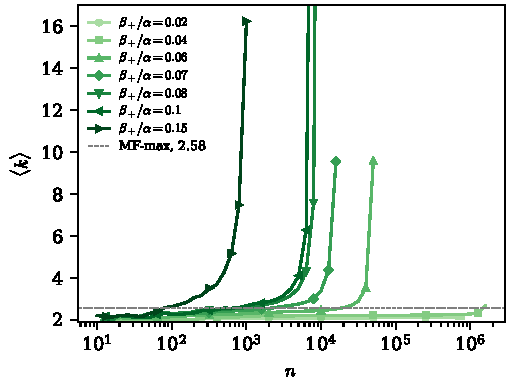
\includegraphics[width=\columnwidth]{fig-pertriad.pdf}
\caption{Mean degree under per-triad rates (closure probability per event
$\beta_+ W/(\alpha N+\beta_+ W)$, uniform open triad). Runs to $10^6$ stop at
$E/N=50$. The longer run at $\beta_+/\alpha=0.04$ was stopped by hand at
$1.6\times10^6$, inside the runaway. Dashed line: the largest stationary mean-field
density, $2.58$.}
\label{fig:pertriad}
\end{figure}

Simulations (Fig.~\ref{fig:pertriad}) show the runaway for
$\beta_+/\alpha\ge0.06$ within $10^3$--$5\times10^4$ nodes. Below it,
$\langle k\rangle$ looks stationary for a while ($2.09$ at $\beta_+/\alpha=0.02$,
$2.23$ at $0.04$). But the plateau at $0.04$ corresponds to an effective
$u=1-2/\langle k\rangle\approx0.10$, for which Sec.~\ref{sec:condensation}
predicts condensation at $n^*\approx2\times10^6$. The run condenses near
$10^6$ and then runs away ($\langle k\rangle=2.67$ at $1.6\times10^6$ and
rising): once a core forms, $W\sim n^{3/2}$, and closures outpace arrivals.
Because condensation appears to occur at every $u>0$, per-triad rates should
have no stationary density at any $\beta_+>0$. Only a fixed ratio of the total
rates, Eq.~\eqref{eq:kmean}, defines a sparse network.

%=====================================================================
\section{Opening closed triads}
\label{sec:opening}

\paragraph*{The process.}
Links are not permanent. The natural reverse of closure picks a \emph{closed}
triad --- a path $a$--$c$--$b$ with $a$ and $b$ linked --- and removes its
closing link $(a,b)$, turning it back into an open triad. In the language of
Ref.~\cite{book}, Ch.~3, this is the transition from a link to a potential link,
$e\to p$, which that chapter neglects. We add it as a third process at total
rate $\beta_-$. Each closure rule gets its mirror image:
\begin{itemize}
\item[(w)] a uniformly random closed triad. A link lies in as many closed
  triads as it has triangles, $t_e$, so the removed link is drawn with
  probability $\propto t_e$;
\item[(p)] a uniformly random link with $t_e\ge1$;
\item[(c), (f)] the local searches of Sec.~\ref{sec:normal}, now looking for a
  \emph{linked} pair.
\end{itemize}
An event is an arrival, a closure or a removal with probabilities proportional
to $\alpha$, $\beta_+$ and $\beta_-$. Removing a link of a triangle never
disconnects the network, so $E\ge N-1$ at all times. The simulation keeps
$t_e$ for every link in a Fenwick tree; with $\beta_-=0$ it reproduces the
earlier runs exactly.

\paragraph*{Density, and a queue.}
If every removal finds a triangle, $E=n(1+r_+-r_-)$ with $r_\pm=\beta_\pm/\alpha$,
and
\begin{equation}
  \langle k\rangle=2(1+\Delta),\qquad \Delta=\frac{\beta_+-\beta_-}{\alpha}.
  \label{eq:kmeanpm}
\end{equation}
For $\beta_-\ge\beta_+$ this would put $\langle k\rangle$ at or below $2$, which
$E\ge N-1$ forbids. Removals then become limited by the triangles available.
Near a tree, each closure creates one triangle and each removal destroys one, so
the triangle count is a queue with arrival rate $\beta_+$ and service rate
$\beta_-$. For $\beta_-<\beta_+$ it grows as $n$. For $\beta_->\beta_+$ it
stays $O(1)$, and a fraction $(\beta_--\beta_+)/\beta_-$ of the removals find
nothing to remove. Measured at $\beta_+=\alpha$ and $n=10^6$, that fraction is
$0.093$, $0.202$, $0.501$, $0.751$, $0.900$ for $\beta_-/\beta_+=1.1$, $1.25$, $2$,
$4$, $10$, against $0.091$, $0.200$, $0.500$, $0.750$, $0.900$. At $\beta_+=\beta_-$
the queue is critical, and $T=317$ at $n=10^6$, of order $\sqrt n$.
Figure~\ref{fig:removal}c shows the transition. $\langle k\rangle-2=2\Delta$
vanishes linearly at $\beta_-=\beta_+$, and $T/N$ drops from $0.75$
($\beta_-/\beta_+=0.5$) to $3\times10^{-4}$ ($1$) and $10^{-5}$ ($1.1$).
So the parameter plane splits first along the diagonal: a sparse network with
extensive triangles for $\beta_+>\beta_-$, and a tree for $\beta_+\le\beta_-$.
Since $\alpha+\beta_++\beta_-$ only sets the clock, the two remaining
parameters can be taken as the net growth $\Delta$, which fixes the density,
and the turnover $\beta_-/\beta_+$.

\paragraph*{The tree phase has no hubs.}
In the tree phase a closure is almost always followed by the removal of one of
the three links of the triangle it made. One time in three this undoes the
closure. The other two times it removes a link at the centre $c$ of the triad
and hands it to one of $c$'s neighbours, so $c$ loses one link. Under rule (w)
the centre is drawn with weight $k_c(k_c-1)$, so a node loses links at a rate
quadratic in its degree and gains them (as a neighbour of a centre) at a rate
linear in it. Degrees are therefore confined. At $\beta_+=\alpha$ and
$\beta_-\ge\beta_+$, $k_{\max}=11$--$13$ at both $n=10^5$ and $10^6$, against
$\log_2 n\approx20$ for a uniform random tree. The ratio $P(k)/P(k-1)$ falls
from $0.6$ at $k=2$ to $0.2$ at $k=10$, where a uniform random tree has a
constant $1/2$. Assortativity is $-0.14$.

\paragraph*{Mean field in the triangle phase.}
For $\beta_+>\beta_-$, a node is an endpoint of a removal with probability
$2t_a/(3T)$ per removal, where $t_a$ is its number of triangles. If clustering
falls as $1/k$, then $t_a\propto k_a$, and the removal term is exactly linear:
\begin{equation}
  n\frac{dk_i}{dn}=1+\frac{2(r_+-r_-)}{\langle k\rangle}k_i
  =1+\Bigl(1-\frac{2}{\langle k\rangle}\Bigr)k_i .
\end{equation}
In the uncorrelated limit turnover changes nothing at fixed density; for
$\langle k\rangle=4$, $\gamma=3$ whatever $\beta_-$. Everything turnover does
must therefore come through correlations, which is where the condensation came
from in the first place.

\begin{figure*}[t]
\includegraphics[width=\textwidth]{fig-removal.pdf}
\caption{Closure plus opening under rule (w). (a) Share of the net closure links
held by the $n^{0.8}$ highest-degree nodes,
$\psi=\phi(n^{0.8})(1+\Delta)/\Delta$, against $\beta_-/\beta_+$. Five
densities, $n=10^5$ (open, dashed), $10^6$ (filled) and $10^7$ (stars). In the
condensed phase $\psi\approx1$ and does not fall with $n$. The band marks the
boundary, $\beta_-/\beta_+=0.80$--$0.86$. (b) Phase diagram; points are the
$n=10^6$ runs, filled where $\psi>0.9$. (c) Crossing $\beta_+=\beta_-$ at
$\beta_+=\alpha$, $n=10^6$: excess degree, triangles per node, and
$k_{\max}/100$. Points with $T=0$ are off the axis.}
\label{fig:removal}
\end{figure*}

\paragraph*{Condensation with turnover.}
Take $\langle k\rangle=4$ ($\Delta=1$, $\beta_+=\alpha+\beta_-$). The dense core
thins out as turnover grows. The share of links among the $\sqrt n$ richest nodes
falls from $0.20$ to $0.09$, $0.02$, $0.005$ and $0.001$ at $\beta_-/\alpha=0$,
$0.5$, $1$, $2$, $4$ ($n=10^6$). The links have not left the rich nodes,
however. The $n^{0.8}$ richest nodes hold $0.52$, $0.52$, $0.52$, $0.51$, $0.49$
of all links, essentially the whole net closure share $\Delta/(1+\Delta)=1/2$, and
these numbers change by less than $0.04$ between $n=10^4$ and $10^6$. Under the local rules,
by contrast, the same fraction falls as in any non-condensed network ($0.27$,
$0.18$, $0.11$ at $n=10^4,10^5,10^6$; $0.15$, $0.09$, $0.05$ for $LS(n,1)$).
Turnover thus dilutes the condensate into a sparse club. Its size $n^{a^*}$,
defined by holding half the net closure links, grows from $a^*\approx0.52$ at
$\beta_-=0$ to $0.73$ at $\beta_-/\alpha=4$, independent of $n$ at fixed
$\beta_-$. The largest degree follows: between $n=10^6$ and $8\times10^6$,
$k_{\max}\sim n^\theta$ with $\theta=0.52$, $0.44$, $0.33$, $0.23$ at
$\beta_-/\alpha=0.5$, $1$, $2$, $4$.

\paragraph*{A second boundary.}
At larger turnover the club dissolves. Figure~\ref{fig:removal}a plots the
normalized share $\psi$ against $\beta_-/\beta_+$ for $\Delta=0.1$--$2$. The
curves for all densities fall together: $\psi\approx1$ up to
$\beta_-/\beta_+=0.8$, then a drop. Beyond it $\psi$
decreases with $n$ as for the local rules, $k_{\max}$ grows slowly ($23$, $26$
at $n=10^5,10^6$ for $\Delta=1$, $\beta_-/\alpha=16$), and the assortativity
falls. This is a third phase: extensive triangles, a density set by
Eq.~\eqref{eq:kmeanpm}, and no condensate (Fig.~\ref{fig:removal}b). Every point at $\beta_-/\beta_+=0.8$ has $\psi$ flat or rising
between $n=10^5$ and $10^6$ (four densities; $\Delta=0.1$ has no such point). Every point at $0.83$ and
above falls. Four points just above the boundary, followed to $n=10^7$, keep
falling and none turns back up: $\psi=0.78$, $0.73$, $0.68$ at $\Delta=1$,
$\beta_-/\beta_+=0.857$; $0.79$, $0.74$, $0.72$ at $\Delta=0.25$; $0.72$, $0.55$,
$0.39$ at $\Delta=0.5$; and $0.49$, $0.35$, $0.23$ at $\Delta=1$ (the last three at
$0.889$), for $n=10^5$, $10^6$, $10^7$. We therefore place the boundary at
$\beta_-/\beta_+=0.80$--$0.86$, the same for all $\Delta$ within that resolution.
Close to it the decay is slow, and with $\beta_-=0$ the onset of condensation
moved to very large $n$ at small $u$. Sizes beyond $10^7$ could still move the
boundary slightly.

\paragraph*{Local rules.}
The friend-of-a-friend rule (f) never condenses. At $\langle k\rangle=4$ its age
exponent stays at $0.31$--$0.34$ for $\beta_-/\alpha=0$ to $4$, the $LS(n,1)$
class, and its mean clustering falls from $0.37$ to $0.12$. On approaching
$\beta_-=\beta_+$ at $\beta_+=\alpha$ its hubs fade ($k_{\max}=95$, $37$, $17$
at $\beta_-/\beta_+=0.5$, $0.8$, $0.9$), and at $\beta_+=\beta_-$ it reaches
the same tree ($k_{\max}=12$). For $\beta_->\beta_+$ we did not simulate the
local rules: their removal search, which starts from a random node, must find
one of $O(1)$ triangles, and that is too slow to run.

%=====================================================================
\section{Discussion}

Holding $\beta_+/\alpha=\langle k\rangle/2-1$ fixes the density. $\beta_+=\alpha$
matches $LS(n,1)$, and $u=\beta_+/(\alpha+\beta_+)$ is the one parameter left.
What the decoupled model builds depends on how the open triad is found:

\begin{itemize}
\item A \emph{local} closure --- a random node introduces two friends, or
  befriends a friend of a friend --- gives a scale-free, clustered network with
  $\gamma=1+2/(eu)$. The friend-of-a-friend version is the faithful
  generalization of $LS(n,1)$: at $\beta_+=\alpha$ it has the same density and the
  same exponent, $\gamma=5$.
\item A \emph{census} closure --- a triad drawn uniformly from the whole
  network --- weights each centre by $k(k-1)$. The resulting feedback condenses
  the network into a near-clique core of order $\sqrt n$ nodes holding a finite
  fraction of the links. The onset size grows roughly as $u^{-5}$, with no
  sign of a finite threshold.
\item \emph{Opening} closed triads at rate $\beta_-$ adds two boundaries. At
  $\beta_-=\beta_+$ triangles become a critical queue: below it they are
  extensive and $\langle k\rangle=2[1+(\beta_+-\beta_-)/\alpha]$, above it the
  network is a tree whose degrees stay bounded. Between the two, at
  $\beta_-/\beta_+\approx0.83$, turnover dissolves the condensate, which before
  that only spreads into a sparse club of $n^{a}$ nodes.
\end{itemize}

The condensation differs from the Bose--Einstein condensation of fitness models
\cite{bianconi2001} and from superlinear preferential attachment
\cite{krapivsky2000}. There a single node captures a finite fraction of the
links; here a growing \emph{dense block} does, and every node in it has degree
$\sim\sqrt n$. In graphon language the network is sparse with a dense spike: a
$\Theta(\sqrt n)$ block of finite density.

\paragraph*{Open questions.}
(i) A controlled theory of the onset: the scaling variable for
$n^*(u)$ (power law versus essential singularity) and the seed-to-seed
distribution of $n^*$. (ii) Whether $\phi$, the core's share of links, has a
limit and how it depends on $u$ (at $n=10^6$, $\phi\approx0.15$--$0.2$ for $0.3\le u\le0.7$; data/scan.csv). (iii) The scaling of the sparse
core under rule (p). (iv) Mixtures of local and census closure, which
should move the onset continuously. (v) Whether the condensate boundary at
$\beta_-/\beta_+\approx0.83$ is a sharp line or drifts towards $1$ with $n$, and
a theory of the club exponent $a^*(\beta_-/\beta_+)$. (vi) The degree
distribution of the tree phase, which the $k^2$ erosion argument should give in
closed form.

\paragraph*{Reproducibility.}
All results come from \texttt{tc.c} (modes \texttt{l, w, p, c, f, r}) in this
folder, with \texttt{scan.py}, \texttt{runs\_ts.sh}, \texttt{runs\_onset.sh},
\texttt{onset.py}, \texttt{scan\_rm.py}, \texttt{runs\_rm\_ts.sh}, \texttt{club.py},
\texttt{cross.py}, \texttt{phase.py} and \texttt{mkfigs.py}. Summaries are in \texttt{data/}.

\begin{thebibliography}{99}
\bibitem{granovetter1973} M. S. Granovetter, Am. J. Sociol. \textbf{78}, 1360 (1973).
\bibitem{davidsen2002} J. Davidsen, H. Ebel, and S. Bornholdt, Phys. Rev. Lett. \textbf{88}, 128701 (2002).
\bibitem{holme2002} P. Holme and B. J. Kim, Phys. Rev. E \textbf{65}, 026107 (2002).
\bibitem{vazquez2003} A. V\'azquez, Phys. Rev. E \textbf{67}, 056104 (2003).
\bibitem{toivonen2006} R. Toivonen, J.-P. Onnela, J. Saram\"aki, J. Hyv\"onen, and K. Kaski, Physica A \textbf{371}, 851 (2006).
\bibitem{jackson2007} M. O. Jackson and B. W. Rogers, Am. Econ. Rev. \textbf{97}, 890 (2007).
\bibitem{vazquez2001} A. V\'azquez, Europhys. Lett. \textbf{54}, 430 (2001).
\bibitem{book} A. V\'azquez, \emph{Local network growth: how simple rules drive network complexity} (2026).
\bibitem{bianconi2001} G. Bianconi and A.-L. Barab\'asi, Phys. Rev. Lett. \textbf{86}, 5632 (2001).
\bibitem{krapivsky2000} P. L. Krapivsky, S. Redner, and F. Leyvraz, Phys. Rev. Lett. \textbf{85}, 4629 (2000).
\end{thebibliography}

\end{document}
